\chapter{Introducción}
\label{cap:capitulo1}
\setcounter{page}{1}

\begin{flushright}
\begin{minipage}[]{10cm}
\emph{La motivación nos impulsa a comenzar y el hábito nos permite continuar}\\
\end{minipage}\\

Jim Ryun\\
\end{flushright}

\vspace{1cm}

La robótica ha sufrido una transformación enorme a lo largo de su historia, aunque siempre teniendo en mente el mismo objetivo: cumplir con el deseo humano. Debido a esa transformación y ese deseo se ha podido consolidar este campo en la actualidad, que abarca cada sector que se pueda imaginar. Otra vertiente que ha destacado en la robótica estos últimos años ha sido la creación de robots de bajo coste para que puedan llegar a un mayor número de personas y se puedan beneficiar de esta ciencia. 

En el presente capítulo se va a abordar el contexto de la robótica, explicando brevemente su historia para poder entender realmente qué es la robótica y lo que es un robot. También se van a encuadrar los tipos de robots que existen y sus múltiples aplicaciones. Todo esto nos ayudará a poder entender mejor dónde se encuadra el presente trabajo, proporcionando los conocimientos necesarios, tanto teóricos como prácticos, que se describirán a lo largo del documento.

\section{La robótica}
\label{sec:robotica} % etiqueta para luego referenciar esta sección

La robótica es el campo de la ingeniería que se enfoca en el diseño, la construcción y la programación de robots. Y un robot se podría definir como un sistema informático formado por sensores y actuadores imprecisos, ya que operan en el mundo real que es imperfecto también. Los robots realizan tareas repetitivas, aburridas y peligrosas, y tienen que ser sensibles al entorno. Sin embargo, no existe una definición unívoca al respecto y depende del campo y de la época de la que queramos hablar. Para poder entenderlo, se va a hacer un breve resumen sobre la historia de la robótica.

Desde la antigüedad se han desarrollado ingenios o autómatas, de los cuáles muchos de ellos tenían fines religiosos, como los mostrados en la Figura \ref{fig:ancientrel}. 


\begin{figure}[ht!]
	\centering
	\begin{minipage}{0.4\linewidth}
		\centering
		\includegraphics[width=\linewidth]{figs/memnon.jpeg}
		\caption*{\centering Estatuas de Memnon $^{\ref{note:enlace1}}$} %\cite{memnon_image}
	\end{minipage}
	\hspace{2cm}
	% aquí incluir iamgen de Guerrero de terracota
	\begin{minipage}{0.35\linewidth}
		\centering
		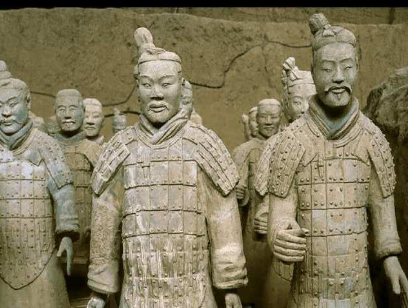
\includegraphics[width=\linewidth]{figs/terracota.png}
		\caption*{\centering Guerreros de Terracota $^{\ref{note:enlace2}}$} %\cite{gomezguerreros}
	\end{minipage}
	\caption{Ingenios de la antigüedad con fines religiosos}
	\label{fig:ancientrel}
\end{figure}


% Definir la primera nota al pie con el número 1
\setcounter{footnote}{1} % Reiniciar la numeración de notas al pie
\footnotetext[\value{footnote}]{\url{https://es.wikipedia.org/wiki/Colosos_de_Memn\%C3\%B3n}\label{note:enlace1}}

\setcounter{footnote}{2} % Reiniciar la numeración de notas al pie
\footnotetext[\value{footnote}]{\url{https://es.wikipedia.org/wiki/Guerreros_de_terracota}\label{note:enlace2}}
 
Otras invenciones que destacaban por otras aplicaciones fueron el tornillo de Arquímedes de Siracusa, la eolípila de Herón de Alejandría, el ornitóptero de Leonardo Da Vinci y el hombre de palo de Juanelo Turriano, entre otras.

En \cite{cuenca2023diseno} se trata el principio de generación hidroeléctrica, tomando en cuenta el modelo tornillo de Arquímedes. También en el artículo \cite{giri2020maquinas} se traza una línea histórica de las máquinas térmicas, teniendo en cuenta a la eolípila. Dichas invenciones aparecen reflejadas en la Figura \ref{fig:ancient}.

\begin{figure}[ht!]
	\centering
	% Imagen del tornillo de Arquímedes de Siracusa
	\begin{minipage}{0.3\linewidth}
		\centering
		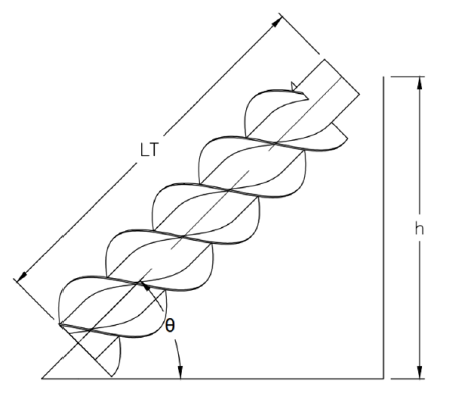
\includegraphics[width=\linewidth]{figs/arquimedes.png}
		\caption*{\centering Tornillo de Arquímedes}  %\cite{cuenca2023diseno}
	\end{minipage}
	\hspace{3cm}
	% Imagen de la eolípila
	\begin{minipage}{0.3\linewidth}
		\centering
		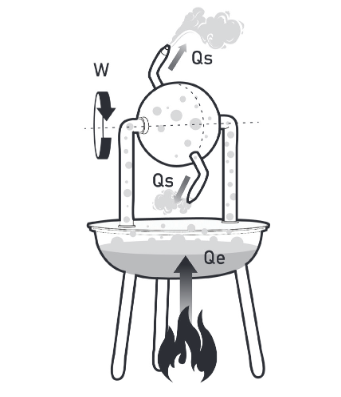
\includegraphics[width=\linewidth]{figs/eolipila.png}
		\caption*{\centering Eolípila} %\cite{giri2020maquinas}
	\end{minipage}
	%\hspace{3cm}
	% Imgen del ornitóptero
	%\begin{minipage}{0.3\linewidth}
	%	\centering
	%	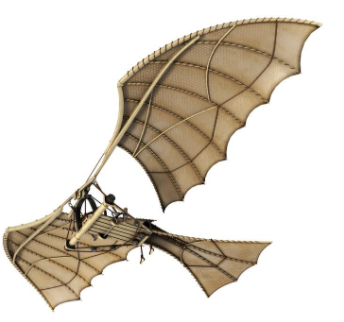
\includegraphics[width=\linewidth]{figs/davinci.png}
	%	\caption*{\centering Ornitóptero \cite{velazquezcual}}
	%\end{minipage}
	%\hspace{3cm}
	% Imagen del hombre de palo 
	%\begin{minipage}{0.3\linewidth}
	%	\centering
	%	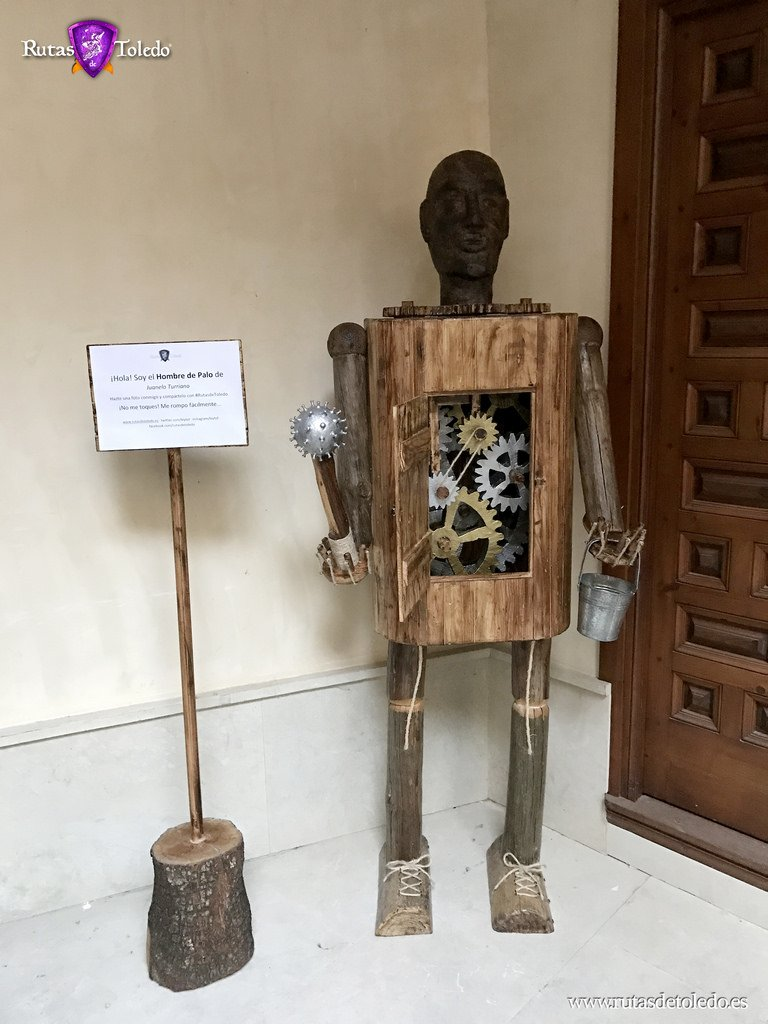
\includegraphics[width=\linewidth]{figs/hombre-palo.jpg}
	%	\caption*{\centering Hombre de palo \cite{hombredepalo_leyendasdetoledo}}
	%\end{minipage}
	\caption{Ingenios de la antigüedad con fines no religiosos}
    \label{fig:ancient}
    \end{figure}

Durante el siglo XX la ciencia dejó de ser una actividad desarrollada en aislamiento y se desarrolló en laboratorios con más gente. El movimiento del positivismo lógico fomentó las investigaciones, ya que este movimiento trataba de dar importancia a la ciencia y dejar de lado la filosofía; también, el contexto de las guerras mundiales y de las bombas nucleares influyeron significativamente en este aspecto. Ya se empieza a acuñar la palabra robot y surge Electro y Sparko de Westinghouse Electric Corporation (Figura \ref{fig:EyS}), tratado en muchas ocasiones como uno de los primeros robots, como se describe en \cite{bidaudrobots}. Un descubrimiento muy destacado fue, y sigue siendo hoy en día, la Leyes de la Robótica de Isaac Asimov, así lo transmite \cite{barcelo2004nuevo}.


\begin{figure} [h!]
	\begin{center}
		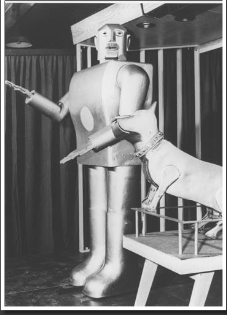
\includegraphics[width=8cm]{figs/electro-sparko.png}
	\end{center}
	\caption{Electro y Sparko} %\cite{bidaudrobots}}
	\label{fig:EyS}
\end{figure}

%\begin{figure} [h!]
%	\begin{center}
%		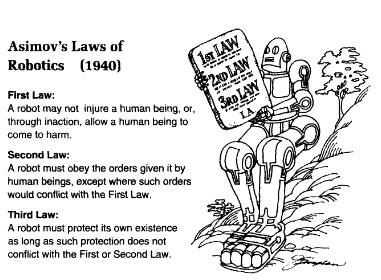
\includegraphics[width=12cm]{figs/issac-law.png}
%	\end{center}
%	\caption{ Leyes de la robótica} %\cite{barcelo2004nuevo}
%\label{fig:Asimov}
%\end{figure}


%\ac{} expande las siglas
%\acs{} no expande las siglas
\cite{nilsson1984shakey} nos cuenta que en 1969 se construye por el \ac{SRI} Internacional un prototipo experimental llamado Shakey, que era una unidad independiente de un metro y medio, equipado con dos motores, cámara de televisión y una radio conectada a un ordenador, capaz de navegar en entornos cerrados y estructurados de una forma autónoma. Sus objetivos eran aprender del medio y ser capaz de planificar trayectorias de movimiento, y las tareas que le asignaron fueron mover y detectar bloques. Sin embargo, cada movimiento podría tardar más de una hora en computarse y, aún así, podrían producirse fallos. A Shakey se le conoce como el primer robot móvil (Figura \ref{fig:sigloxx} izquierda). 

%\begin{figure} [h!]
%	\begin{center}
%		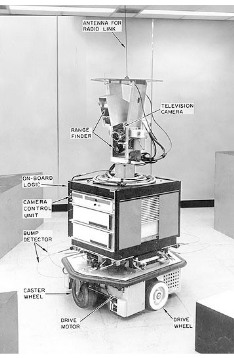
\includegraphics[width=8cm]{figs/shakey.png}
%	\end{center}
%	\caption{Robot Shakey} %\cite{nilsson1984shakey}}
%	\label{fig:shakey}
%\end{figure}


Otro robot muy conocido  y descrito en \cite{earnest2012stanfordcart} es la carreta de Stanford, que era capaz de ver y moverse en cualquier ambiente. Con la cámara que disponía, era capaz de calcular y trazar distancias. Sin embargo, tardaba cinco horas en recorrer treinta metros (Figura \ref{fig:sigloxx} derecha). 

%\begin{figure} [h!]
%	\begin{center}
%		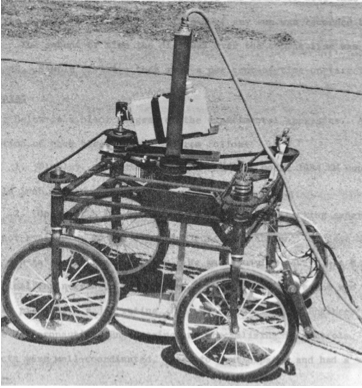
\includegraphics[width=8cm]{figs/stanford.png}
%	\end{center}
%	\caption{Carreta de Stanford}
%	\label{fig:stanford}
%\end{figure}


\begin{figure}[ht!]
	\centering
	% Imagen del tornillo de Arquímedes de Siracusa
	\begin{minipage}{0.35\linewidth}
		\centering
		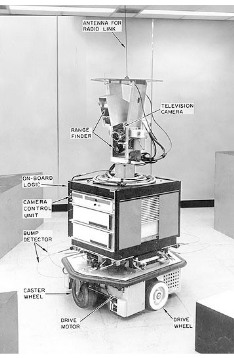
\includegraphics[width=\linewidth]{figs/shakey.png}
		\caption*{\centering Robot Shakey}  %\cite{cuenca2023diseno}
	\end{minipage}
	\hspace{2cm}
	% Imagen de la eolípila
	\begin{minipage}{0.49\linewidth}
		\centering
		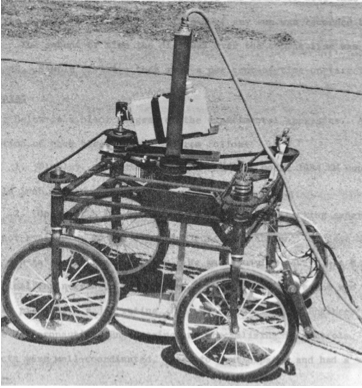
\includegraphics[width=\linewidth]{figs/stanford.png}
		\caption*{\centering Carreta de Stanford}
	\end{minipage}
	\caption{Algunos robots del siglo XX}
	\label{fig:sigloxx}
\end{figure}

Ya a partir de la década de los 80 se decidió que el acceso a los robots fuese para todo el mundo, lo que provocó asombro, inquietud y miedo, ya que el desconocimiento suele generar rechazo. El mundo de la literatura y cine tampoco ayudaba en ese aspecto, ya que se presentaba al robot como algo perjudicial para la humanidad. Afortunadamente, esta situación va menguando con el tiempo, y se está consiguiendo ver a los robots como un asistente del ser humano que lo que quiere es mejorar su calidad de vida. Las dos grandes áreas de investigación centradas en tal propósito son la robótica industrial y la robótica de servicio, que veremos detalladamente a continuación.
%Para conocer en qué ámbitos un robot puede ayudar al ser humano, es necesario conocer que se clasifican en robots industriales y de servicio.


\subsection{Robots industriales}
\label{subsec:robotindustrial}

Los robots industriales son, de forma resumida, brazos robotizados y manipuladores que tienen más de tres grados de libertad, trabajan en entornos controlados y usan efectores como: pinzas, ventosas. etc. Usan control por posición y planificación de trayectorias para poder controlar dichos brazos y poder realizar operaciones como \textit{pick and place}, ensamble de piezas, entre otros. Una variante de los robots industriales son los cobots: capaces de interactuar y colaborar con humanos como se describe en  \cite{ELZAATARI2019162} (Figura \ref{fig:robindustriales} derecha). Dentro del mercado de los robots industriales se puede ver que tiene proveedores asentados como \acs{KUKA}\footnote{\url{https://www.kuka.com/es-es}} o \acs{ABB}\footnote{\url{https://new.abb.com/es}}.



\begin{figure}[ht!]
	\centering
	\begin{minipage}{0.44\linewidth}
		\centering
		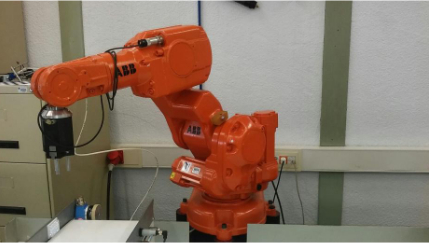
\includegraphics[width=\linewidth]{figs/brazoIRB140.png}
		\caption*{\centering Brazo robot ABB IRB 140 $^{\ref{note:enlace5}}$}

	\end{minipage}
	\hspace{1cm}
	\begin{minipage}{0.4\linewidth}
		\centering
		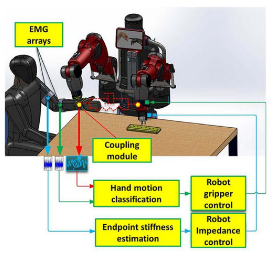
\includegraphics[width=\linewidth]{figs/cobot.png}
		\caption*{\centering Cobot}
		
	\end{minipage}
	\caption{Robots industriales}
	\label{fig:robindustriales}
\end{figure}



\setcounter{footnote}{5} % Establecer la numeración de la siguiente nota al pie
\footnotetext[\value{footnote}]{\url{https://www.youtube.com/watch?v=BBrLAOr89KY}\label{note:enlace5}}


\subsection{Robots de servicio}
\label{subsec:robotservicio}

Los robots de servicios son todos aquellos que no son industriales; por lo tanto, tienen menos de 3 grados de libertad, no trabajan en un entorno controlado, son más difíciles de programar, toman aplicaciones heterogéneas y todavía se encuentran en un mercado inmaduro. Existen muchos tipos de robots de servicio, de los cuáles a continuación se enumeran algunos campos con algunos de sus respectivos ejemplos.


\subsubsection{Robots de limpieza}
\label{subsubsec:robotlimpieza}

En \cite{plaza_robotica_servicio} se define a los robots de limpieza como aquellos robots que se encargan de eliminar la suciedad. Dependiendo de sus características, pueden ser capaces de aspirar y fregar el suelo, o de limpiar los cristales de las ventanas. Estos últimos son comunes en edificios que tienen grandes ventanales y un difícil acceso a ellos. Las aspiradoras se encuentran en un mercado mundial asentado cuyos inicios eran aspiradoras que usaban sensores de contacto, encoders y una navegación pseudoaleatoria (Figura \ref{fig:roblimpieza} izquierda), y han evolucionado hasta el punto de usar mapas para poder navegar y poder localizarse. También usan algoritmos sofisticados, como navegación de cobertura por barridos sistemáticos \acs{BSA}, y se componen de sensores más sofisticados, como láseres y cámaras, que son capaces de detectar obstáculos, como calcetines, y ser capaz de esquivarlos (Figura \ref{fig:roblimpieza} derecha).


\begin{figure}[ht!]
	\centering
	\begin{minipage}{0.3\linewidth}
		\centering
		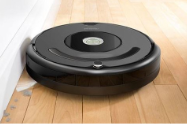
\includegraphics[width=\linewidth]{figs/gama-baja.png}
		\caption*{\centering Modelo económico }% \cite{plaza_robotica_servicio}}
	\end{minipage}
	\hspace{3cm}
	% aquí incluir iamgen de Guerrero de terracota
	\begin{minipage}{0.3\linewidth}
		\centering
		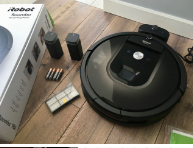
\includegraphics[width=\linewidth]{figs/gama-alta.png}
		\caption*{\centering Gama alta} % \cite{plaza_robotica_servicio}}
	\end{minipage}
	\caption{Robots de limpieza Roomba, de iRobot$^{\ref{note:enlace6}}$}
	\label{fig:roblimpieza}
\end{figure}

\setcounter{footnote}{6} % Establecer la numeración de la siguiente nota al pie
\footnotetext[\value{footnote}]{\url{https://www.irobot.es/}\label{note:enlace6}}

\subsubsection{Robots de entretenimiento}
\label{subsubsec:robotentretenimiento}

Son aquellos robots que tienen aplicaciones heterogéneas en un mercado educativo asentado, pero también existen muchos prototipos sin un uso comercial claro. En educación se ha ido introduciendo la robótica de manera muy atractiva y didáctica a los estudiantes hasta el punto de conseguir tener una asignatura destinada a la robótica y poder participar en competiciones como: \ac{FLL}\footnote{\url{https://firstlegoleague.soy/}}, Robocup Junior\footnote{\url{https://junior.robocup.org/}} y Robocampeones\footnote{\url{https://sites.google.com/view/robocampeonesfuenlabrada/}}, entre otros (Figura \ref{fig:robed} izquierda).  En dicha asignatura se adquieren conocimientos generales de programación, impresión 3D, lógica, introducción a la electrónica y los microcontroladores.

Los prototipos nombrados anteriormente suelen ser demostradores tecnológicos que se crean para exhibiciones, se encuentran a la vanguardia de la tecnología y sirven para atraer un mayor número de clientes como puede ser: Spot de Boston Dynamics, Pepper de Softbank o Sophia de Hanson Robotics. En la Figura \ref{fig:robed} (derecha) se pueden ver un ejemplo de estos demostradores.


\begin{figure}[ht!]
	\centering
	\begin{minipage}{0.35\linewidth}
		\centering
		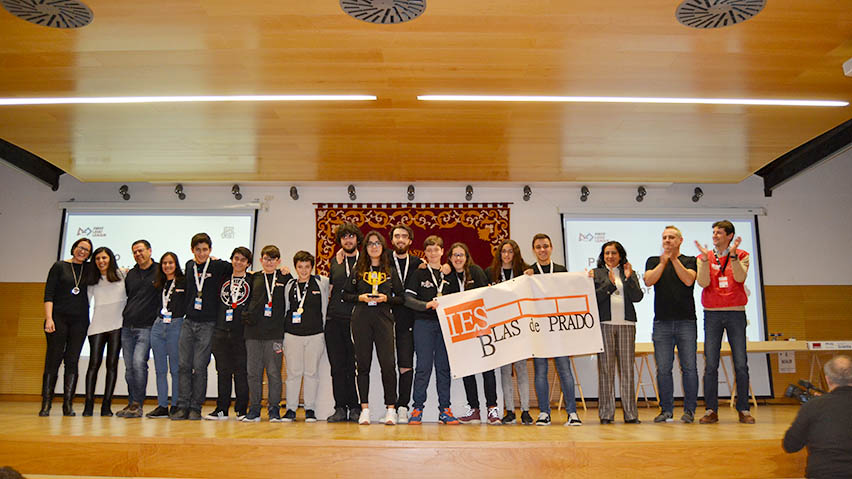
\includegraphics[width=\linewidth]{figs/FLL_TO19.jpg}
		\caption*{\centering \ac{FLL} Toledo $^{\ref{note:enlace10}}$}
	\end{minipage}
	\hspace{3cm}
	% aquí incluir imagen de Spot
	\begin{minipage}{0.3\linewidth}
		\centering
		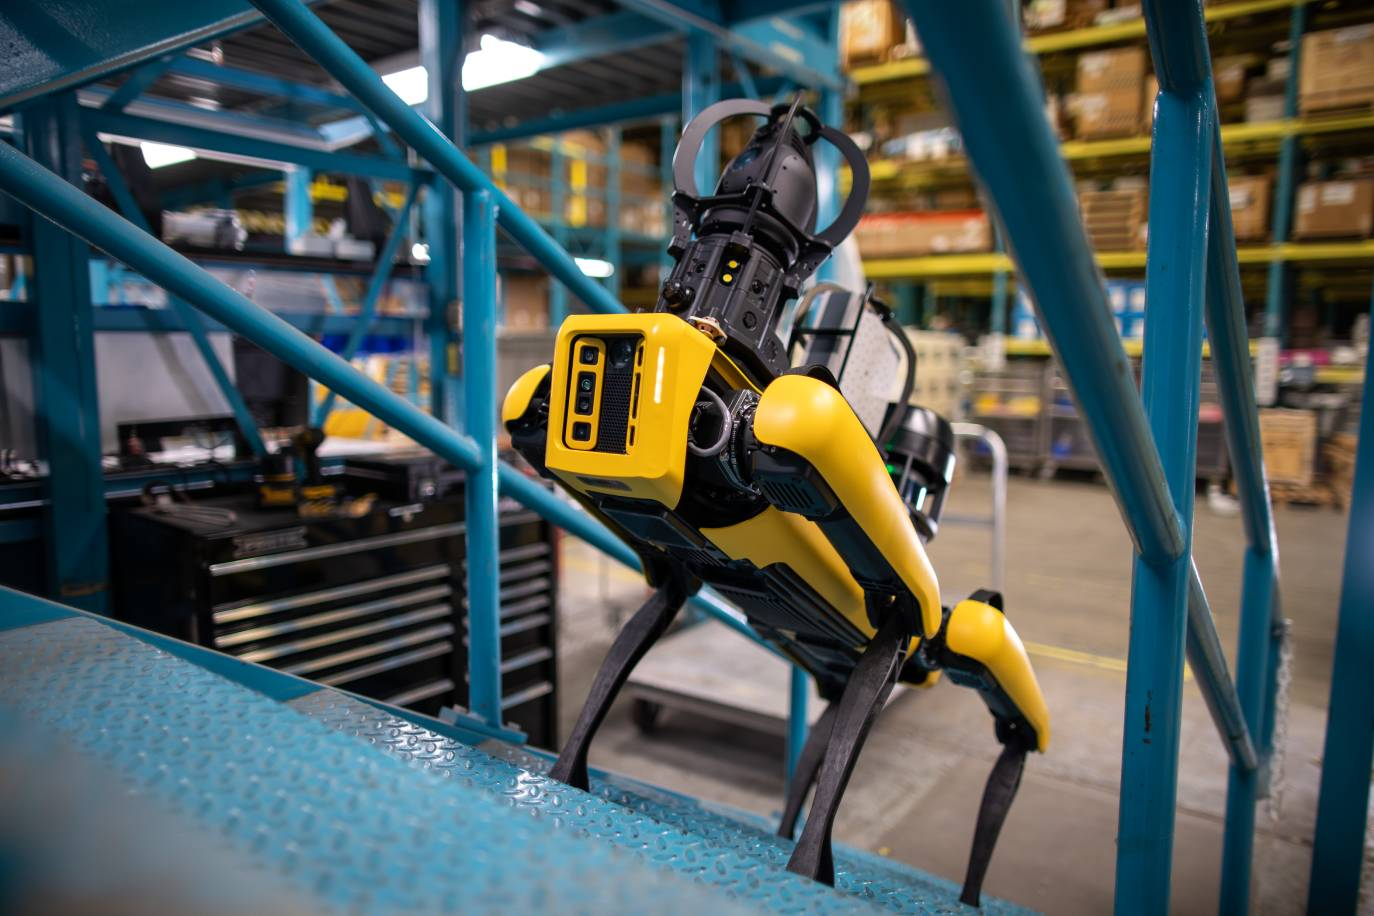
\includegraphics[width=\linewidth]{figs/spot.jpg}
		\caption*{\centering Spot de Boston Dynamics $^{\ref{note:enlace11}}$}
	\end{minipage}
	\caption{Robótica enfocada al entretenimiento}
	\label{fig:robed}
\end{figure}

\setcounter{footnote}{10} % Establecer la numeración de la siguiente nota al pie
\footnotetext[\value{footnote}]{\url{https://www.uclm.es/noticias/febrero2019/toledo/finalfirstlegoleague}\label{note:enlace10}}


\setcounter{footnote}{11} % Establecer la numeración de la siguiente nota al pie
\footnotetext[\value{footnote}]{\url{https://bostondynamics.com/products/spot/}\label{note:enlace11}}

\begin{mdframed}[backgroundcolor=yellow, linecolor=yellow]
\subsubsection{Robots de salud}
\label{subsubsec:robotsalud}


Los robots de salud sirven para mejorar la calidad de la atención médica y apoyar a los profesionales de la salud en diversas tareas. De esas tareas se pueden enumerar las siguientes: telepresencia, asistentes personales, cirugía, desinfección, esterilización, transporte interno y rehabilitación. De este gran abanico de tareas se puede destacar algunas aplicaciones que se puede ver en la Figura \ref{fig:robsalud}.
\end{mdframed}

\begin{figure}[ht!]
	\centering
	\begin{minipage}{0.5\linewidth}
		\centering
		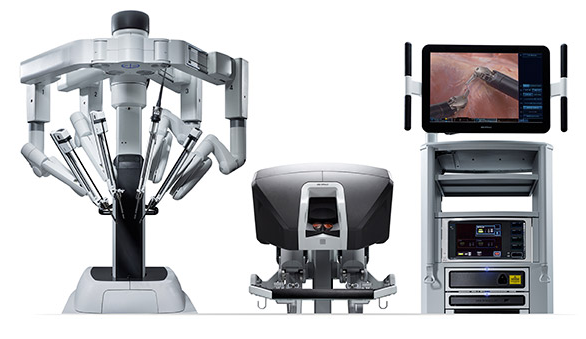
\includegraphics[width=\linewidth]{figs/davincimed.png}
		\caption*{\centering Robot Da Vinci $^{\ref{note:enlace12}}$}
	\end{minipage}
    \hspace{1 cm}
	% aquí incluir imagen de  mako
	\begin{minipage}{0.15\linewidth}
		\centering
		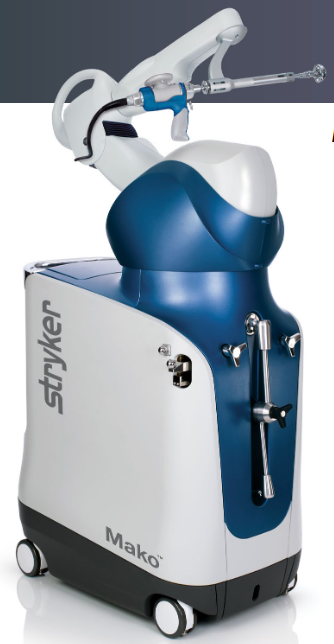
\includegraphics[width=\linewidth]{figs/mako.png}
		\caption*{\centering Robot Mako $^{\ref{note:enlace13}}$}
	\end{minipage}
    \hspace{3cm}
    \begin{minipage}{0.2\linewidth}
    	\centering
    	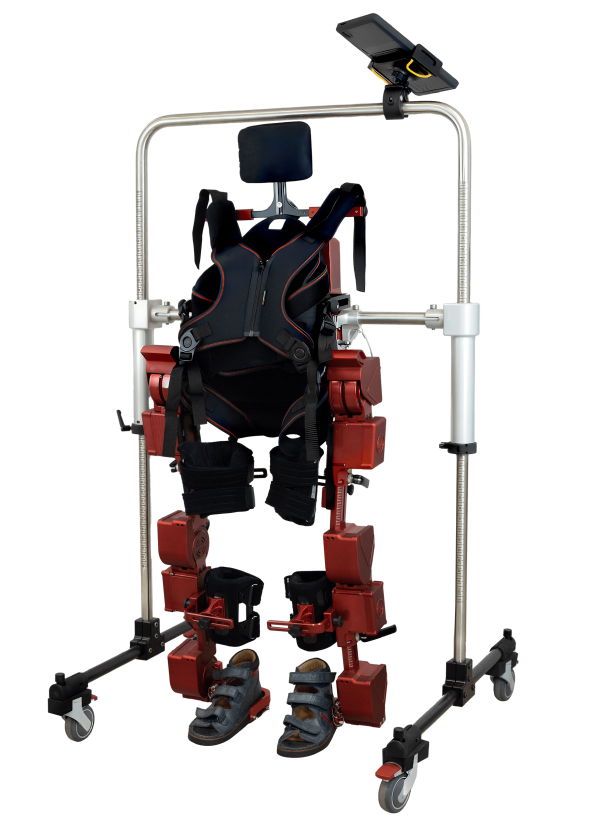
\includegraphics[width=\linewidth]{figs/marsi.png}
    	\caption*{\centering Marsi Bionics $^{\ref{note:enlace14}}$}
    \end{minipage}
    \hspace{3cm}
    \begin{minipage}{0.25\linewidth}
    	\centering
    	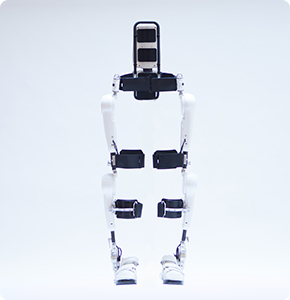
\includegraphics[width=\linewidth]{figs/cyberdyne.jpg}
    	\caption*{\centering CyberDyne $^{\ref{note:enlace15}}$}
    \end{minipage}
	\caption{Robots de salud}
	\label{fig:robsalud}
\end{figure}


\setcounter{footnote}{12} % Establecer la numeración de la siguiente nota al pie
\footnotetext[\value{footnote}]{\url{https://www.abexsl.es/es/sistema-robotico-da-vinci/que-es}\label{note:enlace12}}

\setcounter{footnote}{13} % Establecer la numeración de la siguiente nota al pie
\footnotetext[\value{footnote}]{\url{https://www.stryker.com/content/dam/stryker/joint-replacement/systems/mako-system-overview/resources}\label{note:enlace13}}

\setcounter{footnote}{14} % Establecer la numeración de la siguiente nota al pie
\footnotetext[\value{footnote}]{\url{https://www.marsibionics.com/}\label{note:enlace14}}

\setcounter{footnote}{15} % Establecer la numeración de la siguiente nota al pie
\footnotetext[\value{footnote}]{\url{https://www.cyberdyne.com/}\label{note:enlace15}}

\begin{mdframed}[backgroundcolor=yellow, linecolor=yellow]
\subsubsection{Robots de logística}
\label{subsubsec:robotlogistica}

Los robots de logística son sistemas automatizados diseñados para mejorar la eficiencia, precisión y velocidad en la gestión de la cadena de suministro y operaciones logísticas en cadenas de montaje y almacenes. Generalmente, los sistemas automatizados son flotas de robots a las que se les aplica distintas arquitecturas \textit{software} como puede ser \acs{AGV} o \acs{AMR} para poder realizar la tarea asignada. También existen prototipos de robots de reparto que son capaces de hacer entrega de última milla. La Figura \ref{fig:robreparto}  muestra ejemplos de robots de reparto. 
\end{mdframed}

\begin{figure}[ht!]
	\centering
	\begin{minipage}{0.3\linewidth}
		\centering
		\includegraphics[width=\linewidth]{figs/skypod.png}
		\caption*{\centering Skypod de Exotec $^{\ref{note:enlace16}}$ }
	\end{minipage}
	\hspace{3cm}
	% aquí incluir imagen de Amazon prime air
	\begin{minipage}{0.3\linewidth}
		\centering
		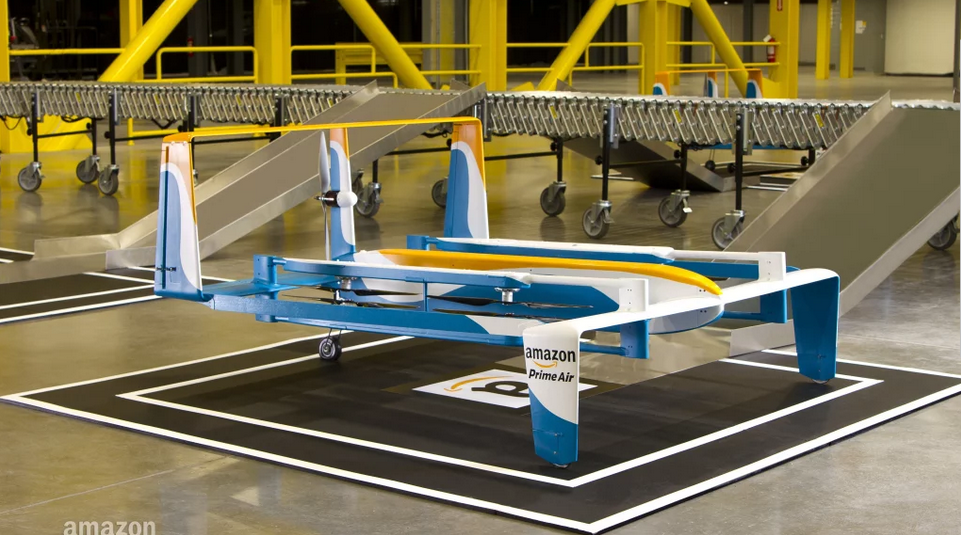
\includegraphics[width=\linewidth]{figs/amazon.png}
		\caption*{\centering Amazon Prime Air $^{\ref{note:enlace17}}$}
	\end{minipage}
	\caption{Robots de logística}
	\label{fig:robreparto}
\end{figure}

\setcounter{footnote}{16} % Establecer la numeración de la siguiente nota al pie
\footnotetext[\value{footnote}]{\url{https://exotecbydexter.com/skypod/}\label{note:enlace16}}


\setcounter{footnote}{17} % Establecer la numeración de la siguiente nota al pie
\footnotetext[\value{footnote}]{\url{https://www.aboutamazon.es/noticias/innovacion/prime-air}\label{note:enlace17}}

\section{Robots de campo}
\label{sec:robotcampo}

En \cite{thorpe2003field} se define a los robots de campo como la automatización de muchas plataformas terrestres, marítimas y aéreas en aplicaciones como la minería, la manipulación de carga, la agricultura, la exploración y explotación submarina, las carreteras, la exploración planetaria, la vigilancia costera y el rescate, entre otros. La robótica de campo se caracteriza por la aplicación de los principios robóticos más avanzados en cuanto a sensado, control y razonamiento en entornos no estructurados y difíciles. El atractivo de la robótica de campo es que es una ciencia desafiante, involucra los últimos principios de ingeniería y diseño de sistemas, y ofrece la verdadera posibilidad de que los principios robóticos hagan una contribución económica y social sustancial en muchas áreas de aplicación diferentes. En general, los robots de campo son plataformas móviles que trabajan al aire libre, a menudo produciendo interacciones fuertes con sus entornos, sin supervisión humana.

En los últimos años se ha podido notar un gran progreso en el desarrollo y la implementación de sistemas robóticos de campo. En la Figura \ref{fig:robcampo} se pueden ver ejemplos al respecto. Por contra, debido a las condiciones que se tienen que someter estos robots, su coste es elevado e imposibilita que su uso se pueda extender a aquellos lugares que necesiten de su servicio y que tienen bajos recursos. Es por esto que existe la creciente necesidad de que, para ciertas aplicaciones que no tienen condiciones tan extremas, se creen robots asequibles que puedan lidiar con determinadas tareas. A continuación veremos este campo de investigación. 


\begin{figure}[ht!]
	\centering
	\begin{minipage}{0.3\linewidth}
		\centering
		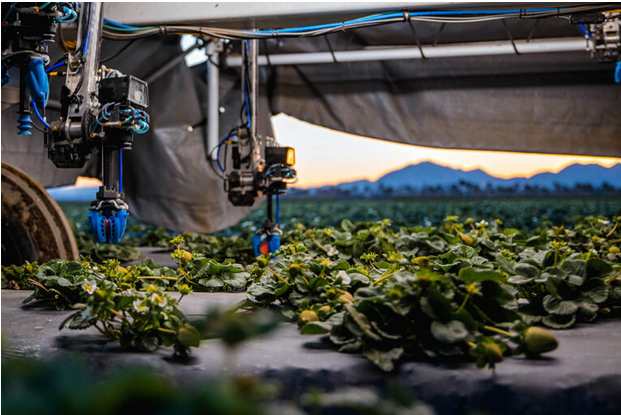
\includegraphics[width=\linewidth]{figs/strawberry.png}
		\caption*{\centering TX Robotic Strawberry Harvester $^{\ref{note:enlace18}}$ }
	\end{minipage}
	\hspace{3 cm}
	% aquí incluir imagen de  mako
	\begin{minipage}{0.3\linewidth}
		\centering
		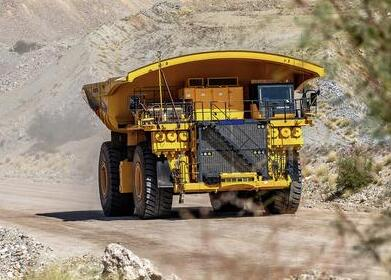
\includegraphics[width=\linewidth]{figs/komatsu.jpeg}
		\caption*{\centering FrontRunner Autonomous Haulage System (AHS) $^{\ref{note:enlace19}}$ }
	\end{minipage}
	\hspace{3cm}
	\begin{minipage}{0.3\linewidth}
		\centering
		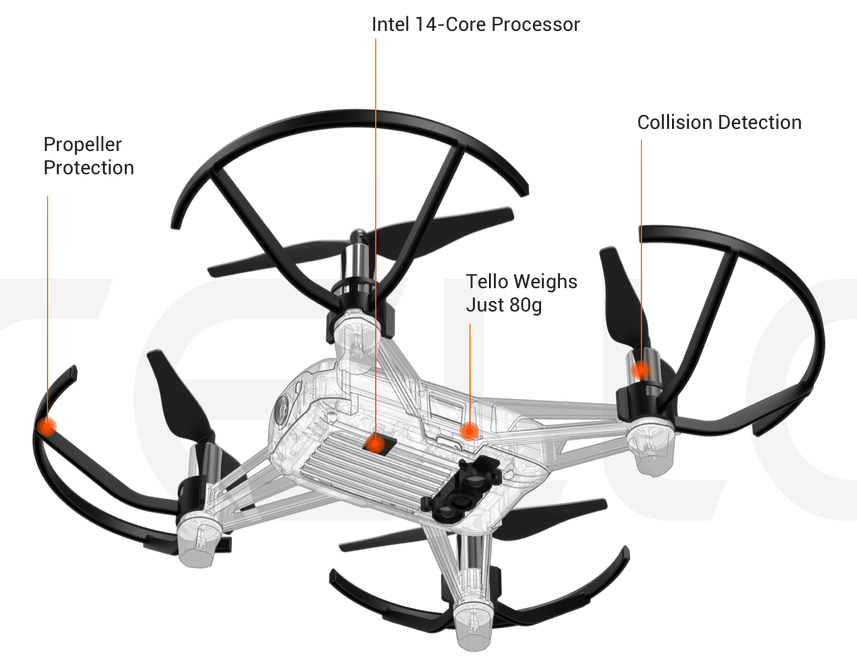
\includegraphics[width=\linewidth]{figs/tello.png}
		\caption*{\centering Drone Tello $^{\ref{note:enlace20}}$ }
	\end{minipage}
	\hspace{3cm}
	\begin{minipage}{0.3\linewidth}
		\centering
		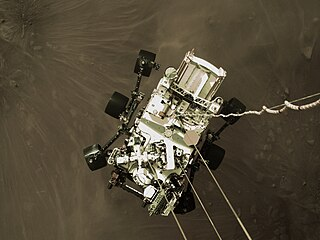
\includegraphics[width=\linewidth]{figs/perseverance.jpg}
		\caption*{\centering Perseverance $^{\ref{note:enlace21}}$ }
	\end{minipage}
	\caption{Robots de campo}
	\label{fig:robcampo}
\end{figure}


\setcounter{footnote}{18} % Establecer la numeración de la siguiente nota al pie
\footnotetext[\value{footnote}]{\url{https://advanced.farm/technology/strawberry-harvester/}\label{note:enlace18}}
\setcounter{footnote}{19} % Establecer la numeración de la siguiente nota al pie
\footnotetext[\value{footnote}]{\url{https://www.komatsu.com/en/technology/smart-mining/loading-and-haulage/autonomous-haulage-system/}\label{note:enlace19}}
\setcounter{footnote}{20} % Establecer la numeración de la siguiente nota al pie
\footnotetext[\value{footnote}]{\url{https://www.ryzerobotics.com/es/tello}\label{note:enlace20}}
\setcounter{footnote}{21} % Establecer la numeración de la siguiente nota al pie
\footnotetext[\value{footnote}]{\url{https://es.wikipedia.org/wiki/Perseverance}\label{note:enlace21}}


\section{Robots de bajo coste}
\label{sec:robotbajocoste}

Los robots de bajo coste son aquellos robots diseñados y fabricados con el objetivo de ser económicos, accesibles y fáciles de producir. Estos robots suelen emplear componentes menos costosos y métodos de fabricación simplificados para reducir el precio final. Algunas características clave de los robots de bajo coste incluyen:

\begin{itemize}
	\item \textit{Componentes asequibles}. Utilizan materiales de propósito general y componentes electrónicos más baratos, coordinados por alguna placa de bajo coste como Arduino o Raspberry Pi.
	\item \textit{Simplicidad en el diseño}. Tienen diseños más sencillos que han sido creados usando técnicas de diseño e impresión 3D, facilitando su actualización y mantenimiento.
	\item \textit{Accesibilidad}. Están diseñados para ser utilizados por cualquier tipo de persona, sin tener una formación avanzada de la materia.
	\item \textit{Educación y prototipos}. Ampliamente usados en educación para facilitar el aprendizaje y también en la creación de prototipos rápidos y asequibles.
	\item \textit{Versatilidad}. Se adaptan a numerosas aplicaciones, desde las más sencillas hasta proyectos más complejos.
	
\end{itemize}\


En resumen, los robots de bajo coste permiten la democratización de la tecnología robótica, facilitando su acceso a un público más amplio y fomentando la innovación y el aprendizaje en diferentes campos. En la Figura \ref{fig:roblowcost} se puede apreciar una aplicación real reciente de la robótica de bajo coste de la universidad \textit{Carnegie Mellon} descrita en el artículo \cite{shaw2024leap}.

\begin{figure} [h!]
	\begin{center}
		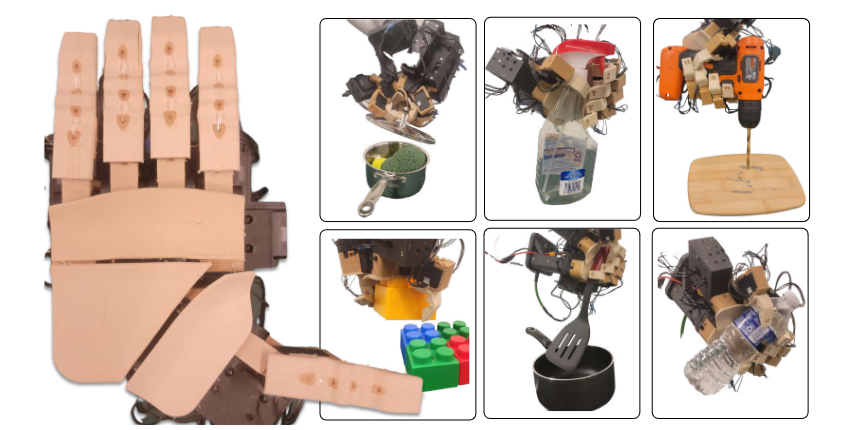
\includegraphics[width=16cm]{figs/handlowcost.png}
	\end{center}
	\caption{Mano Antropomórfica Híbrida Rígida y Suave} %\cite{shaw2024leap}}
	\label{fig:roblowcost}
\end{figure}

%Sabiendo que existen los robots de campo y la robótica de bajo coste, es necesario explorar y conocer las instituciones, los tipos de irregularidades en la carretera y los procesos actuales que existen en España para poder tener un correcto mantenimiento de ellos. 

Con esta base tecnológica, uno de los desafíos donde los robots de bajo coste están mostrando un gran potencial es en tareas repetitivas, como las tareas de mantenimiento, por ejemplo de infraestructuras como las carreteras. A medida que se buscan soluciones más eficientes y económicas para mantener y mejorar las infraestructuras, los robots de bajo coste pueden ser una pieza clave en este proceso.
%los robots de bajo coste pueden abordar problemas globales en campos que requieren soluciones económicas y eficientes, como el mantenimiento de infraestructuras públicas.

El mantenimiento de infraestructuras públicas, y en especial el de las carreteras, es una tarea de vital importancia para garantizar la seguridad y el bienestar de las personas. Sin embargo, también representa un reto logístico y económico significativo. Las carreteras, expuestas constantemente a condiciones climáticas adversas, tráfico pesado y el desgaste natural, requieren un mantenimiento constante para prevenir accidentes y asegurar la movilidad eficiente de personas y mercancías.

Tradicionalmente, este mantenimiento ha dependido de métodos manuales y laboriosos. Equipos de trabajadores inspeccionan las carreteras, identifican los daños y proceden a repararlos, lo que implica un alto coste en tiempo, recursos humanos y materiales. Además, la intervención en las carreteras conlleva cortes de tráfico que generan congestión y molestias tanto para conductores como para peatones.

Aquí es donde la tecnología de los robots de bajo coste puede ofrecer una solución disruptiva. El desarrollo de estos robots ha llegado a un punto en el que pueden ser integrados en el proceso de mantenimiento de carreteras de manera eficaz. Al ser equipados con actuadores, sensores avanzados y algoritmos de \ac{IA}, estos robots tienen la capacidad de detectar y arreglar automáticamente irregularidades en el pavimento, evaluando su tamaño y gravedad. Esta automatización permitiría realizar inspecciones más frecuentes y precisas, reduciendo el margen de error humano, facilitando intervenciones más rápidas y localizadas, y mejorando las condiciones de seguridad de los trabajadores.

La posibilidad de desplegar múltiples robots de bajo coste a lo largo de una red de carreteras también representa una ventaja significativa. Estos robots pueden realizar inspecciones de forma continua, recorriendo largas distancias y detectando problemas antes de que se conviertan en riesgos graves para la seguridad vial. Además, los robots pueden operar en entornos donde el acceso humano es complicado o peligroso, como en carreteras rurales o áreas montañosas.

En este contexto, la versatilidad y el bajo coste de los robots también resultan beneficiosos cuando se trata de reparaciones. Actualmente, las reparaciones suelen ser costosas y temporales, lo que significa que el mismo área puede requerir múltiples intervenciones a lo largo del tiempo. Sin embargo, con robots capaces de aplicar reparaciones rápidas y precisas en el lugar y momento adecuados, se podría reducir la frecuencia de intervenciones costosas y prolongar la vida útil del pavimento. 

Es por todo lo expuesto anteriormente que es necesario conocer la situación de las carreteras en España, conocer qué tipos de deterioros existen, así cómo definir en cuál de todos se va a centrar este proyecto. De este modo, se podrá implementar soluciones innovadoras, como el uso de robots de bajo coste, que no solo optimicen los recursos, sino que también mejoren la seguridad vial y la sostenibilidad del sistema de carreteras a largo plazo.


\section{Conservación de carreteras en España}
\label{sec:conservacioncarreteras}

Según informa el \ac{MITMA}\footnote{\url{https://www.transportes.gob.es/carreteras/catalogo-y-evolucion-de-la-red-de-carreteras}} la red de carreteras de España tiene, a 31 de diciembre de 2023, 165.375 kilómetros, de los cuales 26.473 km forman la \ac{RCE}, que gestiona el \acs{MITMA} y recoge el 52,5\% del tráfico total y el 64,57\% del tráfico pesado. Además, hay 71.145 km que están gestionados por las Comunidades Autónomas y soportan el 42\% del tráfico, y 67.770 km por las Diputaciones (que suponen el 5,5\% del tráfico restante).

España es uno de los países que tiene mayor número de kilómetros de carreteras, y es por ello que tienen que existir distintas entidades que se encarguen de supervisar su mantenimiento. Además de las expuestas previamente, hay varias organizaciones que juegan un papel destacado en la promoción, estudio y mejora continua de las infraestructuras viarias. El \ac{CEDEX}\footnote{\url{https://www.cedex.es/presentacion}}, por ejemplo, es un organismo de referencia en la investigación y experimentación en el ámbito de las obras públicas y la movilidad. Fundado en 1957, el \acs{CEDEX} trabaja para mejorar y conservar las infraestructuras, impulsar una movilidad segura y sostenible, y proteger el medioambiente.

Otra entidad relevante es la \ac{AEC}\footnote{\url{https://www.aecarretera.com/quienes-somos}}, una entidad sin ánimo de lucro fundada en 1949, que trabaja en la defensa y promoción de las carreteras. La \acs{AEC} se enfoca en aspectos como la seguridad vial, la sostenibilidad y la calidad de las infraestructuras, adaptando sus actividades a las necesidades y desafíos contemporáneos, como la digitalización y la descarbonización del transporte.

En el ámbito de la conservación propiamente dicha, la \ac{ACEX}\footnote{\url{https://www.acex.eu/la-asociacion/}}, creada en 1995, agrupa a empresas dedicadas a la conservación de carreteras y se centra en promover la eficiencia y sostenibilidad en el mantenimiento de estas infraestructuras, así como en mejorar la seguridad vial y laboral. También es reseñable destacar sus premios anuales\footnote{\url{https://www.acex.eu/premios-acex/}} que permiten avanzar a pasos agigantados en materia de conservación y seguridad vial.


Sin embargo, parece ser que la labor de todas estas plataformas no es suficiente. Noelia Soage$^{\ref{note:enlace27}}$, redactora en ABC Motor, cuenta que se estuvieron inspeccionando 13.000 kilómetros del total de la red de carreteras de España de las cuáles, se presentan graves deterioros en más del 50\%; los cuales pueden afectar a la estructura o a la superficie de la plataforma, comprometiendo la comodidad, eficiencia y seguridad de la circulación.


Para poder dar mayor contexto a los deterioros, es necesario hacer una clasificación de ellos sabiendo que se pueden presentar en pavimentos flexibles, semiflexibles y semirrígidos urbanos, y los podemos clasificar en cuatro grandes categorías: agrietamiento (Figura \ref{fig:agrietamiento}), degradación del material de la capa de rodadura (Figura \ref{fig:desprendimiento}), degradación de la capa de rodadura sin degradación de material (Figura \ref{fig:deformacion}) y otro tipo de daños (Figura \ref{fig:otro}). \begin{mdframed}[backgroundcolor=yellow, linecolor=yellow] Todo está esquematizado en la Figura \ref{fig:diagrama}.\end{mdframed}

\setcounter{footnote}{27} % Establecer la numeración de la siguiente nota al pie
\footnotetext[\value{footnote}]{\url{https://www.abc.es/motor/reportajes/emisiones-accidentes-aumento-mal-estado-carreteras-senales-20230309230204-nt.html?ref=https}\label{note:enlace27}}

\begin{figure}[H]
	\centering
	\begin{tikzpicture}[node distance=1.5cm, auto,
		every node/.style={text=black, rounded corners=0.05cm},
		grande/.style={rectangle, fill=orange!100!black, font=\large}, 
		peque/.style={rectangle, fill=orange!30!white, font=\large}
		]
		% Nodos principales
		\node[grande] (tipo) {Tipologías de deterioros};
		\node[grande, below of=tipo] (des) {Desprendimiento};
		\node[grande,   left=0.5cm of des] (agri) {Agrietamiento};
		\node[grande,  right=0.25cm of des] (def) {Deformación};
		\node[grande,  right=0.5cm of def] (otro) {Otros tipos};
		
		% subnodos de agrietamiento
		\node[peque, below of=agri] (glon) {grietas longitudinales};
		\node[peque, below of=glon] (gtran) {grietas transversales};
		\node[peque, below of=gtran] (gpc) {grietas piel de cocodrilo};
		
		%subnodos de desprendimiento
		\node[peque, below of=des] (bache) {bache};
		\node[peque, below of=bache] (meteo) {meteorización};
		\node[peque, below of=meteo] (blandon) {blandón};
		\node[peque, below of=blandon] (hueco) {hueco};
		
		%subnodos de deformación
		\node[peque, below of=def] (rod) {roderas};
		\node[peque, below of=rod] (abo) {abombamiento};
		\node[peque, below of=abo] (amp) {ampolla};
		\node[peque, below of=amp] (art) {arrollamiento transversal};
		\node[peque, below of=art] (ond) {ondulaciones};
		\node[peque, below of=ond] (dep) {depresiones};
		
		%subnodos de otros tipos
		\node[peque, below of=otro] (ex) {exudación};
		\node[peque, below of=ex] (parcheo) {parcheo};		
		
		% flechas principales
		\draw[] (tipo) -- (agri);
		\draw[] (tipo) -- (des);
		\draw[] (tipo) -- (def);
		\draw[] (tipo) -- (otro);
		
		% flechas de agrietamiento
		\draw[] (agri) -- (glon);
		\draw[] (glon) -- (gtran);
		\draw[] (gtran) -- (gpc);
		
		% flechas de desprendimiento
		\draw[] (des) -- (bache);
		\draw[] (bache) -- (meteo);
		\draw[] (meteo) -- (blandon);
		\draw[] (blandon) -- (hueco);
		
		% flechas de deformación
		\draw[] (def) -- (rod);
		\draw[] (rod) -- (abo);
		\draw[] (abo) -- (amp);
		\draw[] (amp) -- (art);
		\draw[] (art) -- (ond);
		\draw[] (ond) -- (dep);
		
		% flechas de otros tipos 
		\draw[] (otro) -- (ex);
		\draw[] (ex) -- (parcheo);
		
		
	\end{tikzpicture}
	\caption{Clasificación de deterioros}
	\label{fig:diagrama}
\end{figure}


\begin{figure}[ht!]
	\centering
	\begin{minipage}{0.3\linewidth}
		\centering
		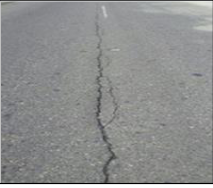
\includegraphics[width=\linewidth]{figs/glon.png}
		\caption*{\centering Grietas longitudinales }
	\end{minipage}
	\hspace{0.5 cm}
	% aquí incluir imagen de  mako
	\begin{minipage}{0.3\linewidth}
		\centering
		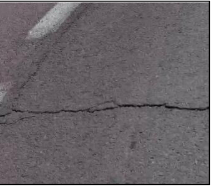
\includegraphics[width=\linewidth]{figs/gtran.png}
		\caption*{\centering Grietas transversales }
	\end{minipage}
	\hspace{0.5 cm}
	\begin{minipage}{0.3\linewidth}
		\centering
		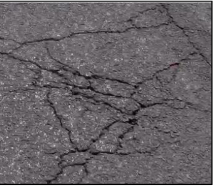
\includegraphics[width=\linewidth]{figs/gpc.png}
		\caption*{\centering Grietas piel de cocodrilo}
	\end{minipage}
	
	\caption{Agrietamiento}
	\label{fig:agrietamiento}
\end{figure}


\begin{figure}[ht!]
	\centering
	\begin{minipage}{0.3\linewidth}
		\centering
		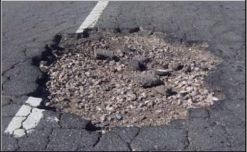
\includegraphics[width=\linewidth]{figs/bache.png}
		\caption*{\centering Bache}
	\end{minipage}
	\hspace{3 cm}
	% aquí incluir imagen de  mako
	\begin{minipage}{0.3\linewidth}
		\centering
		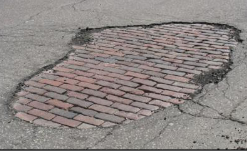
\includegraphics[width=\linewidth]{figs/meteo.png}
		\caption*{\centering Meteorización}
	\end{minipage}
	\hspace{3 cm}
	\begin{minipage}{0.3\linewidth}
		\centering
		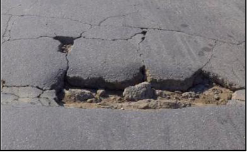
\includegraphics[width=\linewidth]{figs/blandon.png}
		\caption*{\centering Blandón}
	\end{minipage}
	\hspace{3 cm}
	\begin{minipage}{0.3\linewidth}
		\centering
		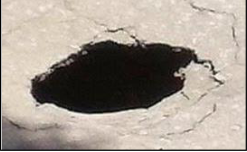
\includegraphics[width=\linewidth]{figs/hueco.png}
		\caption*{\centering Hueco}
	\end{minipage}
	
	\caption{Degradación del material de la capa de rodadura}
	\label{fig:desprendimiento}
\end{figure}


\begin{figure}[ht!]
	\centering
	\begin{minipage}{0.3\linewidth}
		\centering
		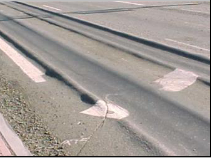
\includegraphics[width=\linewidth]{figs/rod.png}
		\caption*{\centering Roderas }
	\end{minipage}
	\hspace{0.5 cm}
	% aquí incluir imagen de  mako
	\begin{minipage}{0.3\linewidth}
		\centering
		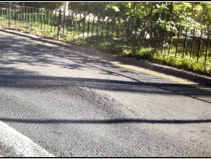
\includegraphics[width=\linewidth]{figs/abo.png}
		\caption*{\centering Abombamiento }
	\end{minipage}
	\hspace{0.5 cm}
	\begin{minipage}{0.3\linewidth}
		\centering
		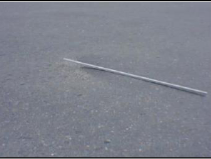
\includegraphics[width=\linewidth]{figs/amp.png}
		\caption*{\centering Ampolla}
	\end{minipage}
	\hspace{0.5 cm}
	\begin{minipage}{0.3\linewidth}
		\centering
		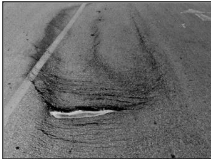
\includegraphics[width=\linewidth]{figs/art.png}
		\caption*{\centering Arrollamiento transversal }
	\end{minipage}
	\hspace{0.5 cm}
	% aquí incluir imagen de  mako
	\begin{minipage}{0.3\linewidth}
		\centering
		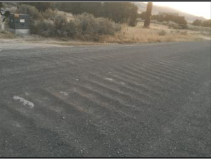
\includegraphics[width=\linewidth]{figs/ond.png}
		\caption*{\centering Ondulaciones }
	\end{minipage}
	\hspace{0.5 cm}
	\begin{minipage}{0.3\linewidth}
		\centering
		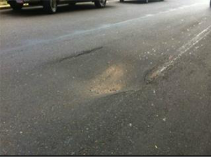
\includegraphics[width=\linewidth]{figs/dep.png}
		\caption*{\centering Depresiones}
	\end{minipage}
	
	
	\caption{Deformación de la capa de rodadura sin degradación de material}
	\label{fig:deformacion}
\end{figure}


\begin{figure}[ht!]
	\centering
	\begin{minipage}{0.3\linewidth}
		\centering
		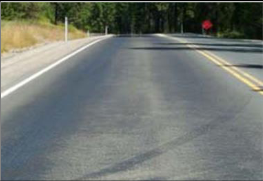
\includegraphics[width=\linewidth]{figs/ex.png}
		\caption*{\centering Exudación }
	\end{minipage}
	\hspace{3 cm}
	% aquí incluir imagen de  mako
	\begin{minipage}{0.3\linewidth}
		\centering
		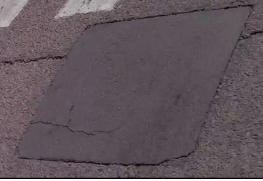
\includegraphics[width=\linewidth]{figs/parcheo.png}
		\caption*{\centering Parcheo }
	\end{minipage}
	
	\caption{Otro tipo de daños}
	\label{fig:otro}
\end{figure}

Tras haber mostrado los tipos de deterioros que existen, nos centramos en el mantenimiento de uno de ellos, ya que el problema es muy grande e intentar tratar todos los casos se torna inabarcable para este proyecto. Así, de todos los tipos mostrados, se van a tratar los baches.\\\\\\  % hay 3 saltos de página

Una vez conocido el deterioro en que se va a centrar este proyecto, los organismos existentes en España y todas las oportunidades que un robot \textit{low-cost} ofrece para el mantenimiento de carreteras, se puede decir que este proyecto se centra en el desarrollo de un robot de campo de tamaño compacto y bajo coste, diseñado para ser fácil de usar y controlar. El robot ha sido fabricado completamente mediante impresión 3D y está equipado con herramientas ampliamente utilizadas en el campo de la robótica. Esta combinación permite que cualquier persona, incluso sin un conocimiento profundo en robótica, pueda replicar el robot y ponerlo en funcionamiento. En el próximo capítulo, se presentarán diversos prototipos y futuras aplicaciones que guardan una cierta relación con el tipo de robot desarrollado.

%La conservación de las carreteras es un aspecto fundamental para garantizar la seguridad vial, la eficiencia del transporte y la durabilidad de las infraestructuras viarias. En España, donde la red de carreteras juega un papel crucial en la conectividad y el desarrollo económico, el mantenimiento adecuado de estas infraestructuras es vital para asegurar un tránsito seguro y fluido, así como para prevenir accidentes y reducir los costos derivados del deterioro del pavimento.

%España cuenta con una extensa red de carreteras que incluye autopistas, autovías, carreteras nacionales, autonómicas, y provinciales. Cada una de estas vías requiere un enfoque específico en cuanto a su mantenimiento y conservación, dado que las condiciones de uso y los desafíos asociados varían considerablemente.

%La conservación de las carreteras en el país está regulada y gestionada por diversas instituciones y organismos. La Dirección General de Carreteras\footnote{\url{https://www.transportes.gob.es/carreteras/organizacion-y-funciones/secretaria-general-de-infraestructuras/direccion-general-de-carreteras}}, bajo la gestión del \ac{MITMA}, es la entidad responsable de la Red de Carreteras del Estado, que incluye las vías de mayor envergadura y tráfico. Por su parte, las comunidades autónomas y las diputaciones provinciales gestionan las carreteras que pertenecen a sus respectivas jurisdicciones, como es el caso de las carreteras autonómicas de Castilla-La Mancha\footnote{\url{https://www.castillalamancha.es/gobierno/fomento/estructura/dgfcartra/actuaciones/cat\%C3\%A1logo-y-mapa-de-carreteras-de-castilla-la-mancha}} y las carreteras provinciales de Toledo\footnote{\url{http://eiel.diputoledo.es/visor/index.php}} .

%Además, varias organizaciones juegan un papel destacado en la promoción, estudio y mejora continua de las infraestructuras viarias. El \ac{CEDEX}\footnote{\url{https://www.cedex.es/presentacion}}, por ejemplo, es un organismo de referencia en la investigación y experimentación en el ámbito de las obras públicas y la movilidad. Fundado en 1957, el \acs{CEDEX} trabaja para mejorar y conservar las infraestructuras, impulsar una movilidad segura y sostenible, y proteger el medioambiente.

%Otra entidad relevante es la \ac{AEC}\footnote{\url{https://www.aecarretera.com/quienes-somos}}, una entidad sin ánimo de lucro fundada en 1949, que trabaja en la defensa y promoción de las carreteras. La \acs{AEC} se enfoca en aspectos como la seguridad vial, la sostenibilidad y la calidad de las infraestructuras, adaptando sus actividades a las necesidades y desafíos contemporáneos, como la digitalización y la descarbonización del transporte.


%En el ámbito de la conservación propiamente dicha, la \ac{ACEX}\footnote{\url{https://www.acex.eu/la-asociacion/}}, creada en 1995, agrupa a empresas dedicadas a la conservación de carreteras y se centra en promover la eficiencia y sostenibilidad en el mantenimiento de estas infraestructuras, así como en mejorar la seguridad vial y laboral. También es reseñable destacar sus premios anuales\footnote{\url{https://www.acex.eu/premios-acex/}} que permiten avanzar a pasos agigantados en materia de conservación y seguridad vial.


%Finalmente, cabe destacar la labor de la Plataforma de Trabajadores de Conservación de Carreteras\footnote{\url{https://conservacion.es/index.php?option=com_content&view=article&id=1&Itemid=101}}, un grupo independiente que agrupa a profesionales del sector preocupados por la seguridad laboral, la reducción de la siniestralidad en las actividades de conservación viaria y por mejorar sus condiciones laborales.\\

%Tras conocer a todos los actores que conforman parte del mantenimiento correcto de las carreteras de España, es necesario conocer los tipos de deterioros del pavimento que se tienen que enfrentar.


%\section{Deterioros del pavimento}

%En el artículo \cite{llopis2020deterioros} se presentan los distintos tipos de deterioros o daños en diferentes tipos de pavimentos, así como su rehabilitación y mantenimento. 

%Para entender las distintas categorías de deterioros, es necesario conocer qué es el firme de una carretera y de qué capas está compuesto. El firme es un conjunto de varias capas de materiales seleccionados y, en la mayoría de los casos, tratados, que forman la superestructura de la plataforma. Su propósito es soportar las cargas del tráfico y garantizar que la circulación se realice de manera segura y cómoda. (Figura \ref{fig:firme})

%\begin{figure} [h!]
%	\begin{center}
%		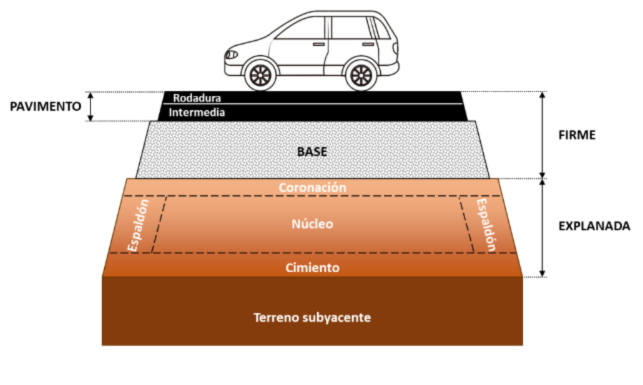
\includegraphics[width=16cm]{figs/firme.png}
%	\end{center}
%	\caption{Firme de una carretera} %\cite{shaw2024leap}}
%\label{fig:firme}
%\end{figure}

%El firme se compone de tres capas: rodadura, capa intermedia y capa base. Las dos primeras forman el pavimento, que soporta las cargas del tráfico y proporciona características como resistencia al deslizamiento y una superficie regular. La capa base, en cambio, tiene una función estructural al absorber las presiones transmitidas y proteger la subbase de cargas excesivas.

%Los firmes se dividen en cuatro tipos: flexibles, semiflexibles, semirrígidos y rígidos. Los firmes flexibles y semiflexibles tienen una capa bituminosa sobre capas granulares. Si el espesor de la capa bituminosa es menor de 15 cm, el firme es flexible; si es mayor, es semiflexible. Los firmes semirrígidos cuentan con un pavimento bituminoso sobre capas tratadas con conglomerantes hidráulicos, con un espesor mínimo de 20 cm. Finalmente, los firmes rígidos tienen un pavimento de hormigón sobre una capa de zahorras.

%\subsubsection{Tipos de deterioros}

%Los distintos tipos de deterioros o daños más comunes que se pueden presentar en
%pavimentos flexibles, semiflexibles y semirrígidos urbanos los podemos clasificar en cuatro grandes categorías: \textit{agrietamiento} (Figura \ref{fig:agrietamiento}), \textit{degradación del material de la capa de rodadura} (Figura \ref{fig:desprendimiento}), \textit{degradación de la capa de rodadura sin degradación de material} (Figura \ref{fig:deformacion}) y \textit{otro tipo de daños} (Figura \ref{fig:otro}). Todo está esquematizado en la Figura \ref{fig:diagrama}.

%%% Incluir aquí las imágenes puestas más arriba 

%Tras haber mostrado toda la gran cantidad de tipos de deterioros que existen, es necesario centrarnos en ser capaces del mantenimiento de uno de ellos ya que el problema es muy grande y sería inabarcable para este proyecto. De todos los tipos mostrados, se van a tratar los \textit{baches}.\\

%\subsubsection{Mantenimiento de baches}

%La reparación de baches en los pavimentos de asfalto es un proceso importante para mantener las carreteras en buen estado. Un bache es una depresión en la superficie de la carretera que puede ser causada por una variedad de factores, como el tráfico pesado, el clima extremo y el envejecimiento del pavimento. Si se dejan sin reparar, los baches pueden causar daños a los vehículos y crear un peligro para los conductores.

%El proceso de reparación de baches comienza con la eliminación del material dañado. Esto se hace mediante el corte del área afectada con una sierra de asfalto o una fresadora. Una vez que se ha eliminado el material dañado, se limpia la superficie hasta dejar el hueco con forma de cuadrilátero regular y se aplica una capa de asfalto fresco. El asfalto se compacta y se alisa para que se ajuste perfectamente al pavimento existente. El resultado final es una superficie de carretera lisa y sin baches\footnote{\url{https://www.youtube.com/watch?v=YPx1bIywgzo}}. En la Figura \ref{fig:repararbache} se puede ver a dos operarios arreglando un bache con asfalto en frío.


%\begin{figure} [h!]
%\begin{center}
%	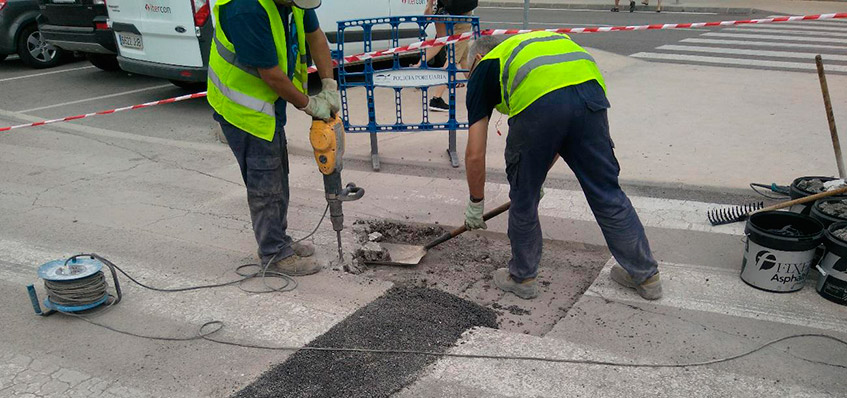
\includegraphics[width=8cm]{figs/repararbache.jpg}
%\end{center}
%\caption{Operarios reparando un bache  $^{\ref{note:reba}}$} %\cite{bidaudrobots}}
%\label{fig:repararbache}
%\end{figure}


%\setcounter{footnote}{30} % Establecer la numeración de la siguiente nota al pie
%\footnotetext[\value{footnote}]{\url{https://fixer.es/blog/como-reparar-bache-con-asfalto-en-frio/}\label{note:reba}}


%Este proyecto se centra en el desarrollo de un robot de campo de tamaño compacto y bajo coste, diseñado para ser fácil de usar y controlar. El robot ha sido fabricado completamente mediante impresión 3D y está equipado con herramientas ampliamente utilizadas en el campo de la robótica. Esta combinación permite que cualquier persona, incluso sin un conocimiento profundo en robótica, pueda replicar el robot y ponerlo en funcionamiento. En el próximo capítulo, se presentarán diversos prototipos y futuras aplicaciones que guardan una cierta relación con el tipo de robot desarrollado.\\
